\section{Part 3 - Prediction Models}

Using \href{https://pandas.pydata.org/}{Pandas} and \href{https://scikit-learn.org/stable/index.html}{Scikit-Learn}
we have create 3 different classification models:

\begin{itemize}
    \item K-Nearest Neighbour.
    \item Decision Trees.
    \item Random Forests.
\end{itemize}

Then using the original dataset we've calculated the accuracy of the predictions and iteratively adjusted each
model's attributes until we obtained the best results for each.

In this section we present the results, and we observe how the \textbf{Random Forest classification algorithm
yields the most accurate prediction results}.

\subsection{K-Nearest Neighbour}

\small
\begin{tabularx}{\linewidth}[H]{| X | X | X | X | X |}
    \caption{K-Nearest Neighbour: Classification report}\label{classification-report-k-nearest} \\
    \hline
    \textbf{Disease} & \textbf{Precision} & \textbf{Recall} & \textbf{F1-score} & \textbf{Support} \\
    \hline
    No & 0.71 & 0.80 & 0.75 & 81 \\
    Yes & 0.85 & 0.77 & 0.81 & 119 \\
    \hline
\end{tabularx}
\normalsize

\begin{figure}[h]
    \caption{K-Nearest Neighbour: Confusion matrix}\label{confusion-matrix-k-nearest}
    \centering
    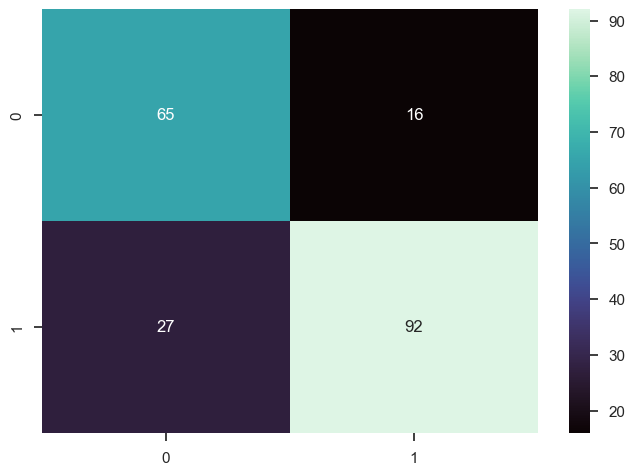
\includegraphics[width=\linewidth]{media/prediction-01-kneighbors.png}
\end{figure}

\subsection{Decision Trees}

\small
\begin{tabularx}{\linewidth}[H]{| X | X | X | X | X |}
    \caption{Decision Trees: Classification report}\label{classification-report-decision-tree} \\
    \hline
    \textbf{Disease} & \textbf{Precision} & \textbf{Recall} & \textbf{F1-score} & \textbf{Support} \\
    \hline
    No & 0.95 & 0.91 & 0.93 & 81 \\
    Yes & 0.94 & 0.97 & 0.95 & 119 \\
    \hline
\end{tabularx}
\normalsize

\begin{figure}[h]
    \caption{Decision Trees: Confusion matrix}\label{confusion-matrix-decision-tree}
    \centering
    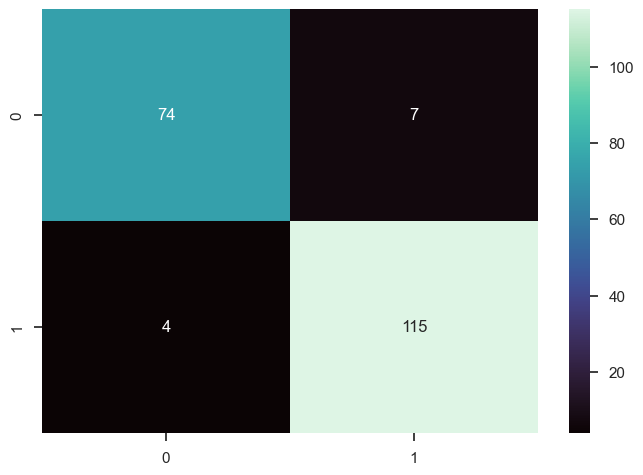
\includegraphics[width=\linewidth]{media/prediction-02-tree.png}
\end{figure}

\subsection{Random Forest}

\small
\begin{tabularx}{\linewidth}[H]{| X | X | X | X | X |}
    \caption{Random Forest: Classification report}\label{classification-report-random-forest} \\
    \hline
    \textbf{Disease} & \textbf{Precision} & \textbf{Recall} & \textbf{F1-score} & \textbf{Support} \\
    \hline
    No & 1.00 & 0.98 & 0.99 & 81 \\
    Yes & 0.98 & 1.00 & 0.99 & 119 \\
    \hline
\end{tabularx}
\normalsize

\begin{figure}[h]
    \caption{Random Forest: Confusion matrix}\label{confusion-matrix-random-forest}
    \centering
    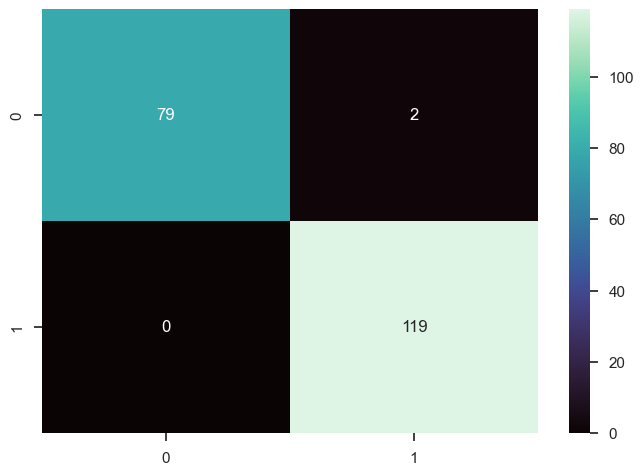
\includegraphics[width=\linewidth]{media/prediction-03-forest.png}
\end{figure}